% Options for packages loaded elsewhere
\PassOptionsToPackage{unicode}{hyperref}
\PassOptionsToPackage{hyphens}{url}
%
\documentclass[
]{article}
\usepackage{amsmath,amssymb}
\usepackage{iftex}
\ifPDFTeX
  \usepackage[T1]{fontenc}
  \usepackage[utf8]{inputenc}
  \usepackage{textcomp} % provide euro and other symbols
\else % if luatex or xetex
  \usepackage{unicode-math} % this also loads fontspec
  \defaultfontfeatures{Scale=MatchLowercase}
  \defaultfontfeatures[\rmfamily]{Ligatures=TeX,Scale=1}
\fi
\usepackage{lmodern}
\ifPDFTeX\else
  % xetex/luatex font selection
\fi
% Use upquote if available, for straight quotes in verbatim environments
\IfFileExists{upquote.sty}{\usepackage{upquote}}{}
\IfFileExists{microtype.sty}{% use microtype if available
  \usepackage[]{microtype}
  \UseMicrotypeSet[protrusion]{basicmath} % disable protrusion for tt fonts
}{}
\makeatletter
\@ifundefined{KOMAClassName}{% if non-KOMA class
  \IfFileExists{parskip.sty}{%
    \usepackage{parskip}
  }{% else
    \setlength{\parindent}{0pt}
    \setlength{\parskip}{6pt plus 2pt minus 1pt}}
}{% if KOMA class
  \KOMAoptions{parskip=half}}
\makeatother
\usepackage{xcolor}
\usepackage[margin=2.54cm]{geometry}
\usepackage{color}
\usepackage{fancyvrb}
\newcommand{\VerbBar}{|}
\newcommand{\VERB}{\Verb[commandchars=\\\{\}]}
\DefineVerbatimEnvironment{Highlighting}{Verbatim}{commandchars=\\\{\}}
% Add ',fontsize=\small' for more characters per line
\usepackage{framed}
\definecolor{shadecolor}{RGB}{248,248,248}
\newenvironment{Shaded}{\begin{snugshade}}{\end{snugshade}}
\newcommand{\AlertTok}[1]{\textcolor[rgb]{0.94,0.16,0.16}{#1}}
\newcommand{\AnnotationTok}[1]{\textcolor[rgb]{0.56,0.35,0.01}{\textbf{\textit{#1}}}}
\newcommand{\AttributeTok}[1]{\textcolor[rgb]{0.13,0.29,0.53}{#1}}
\newcommand{\BaseNTok}[1]{\textcolor[rgb]{0.00,0.00,0.81}{#1}}
\newcommand{\BuiltInTok}[1]{#1}
\newcommand{\CharTok}[1]{\textcolor[rgb]{0.31,0.60,0.02}{#1}}
\newcommand{\CommentTok}[1]{\textcolor[rgb]{0.56,0.35,0.01}{\textit{#1}}}
\newcommand{\CommentVarTok}[1]{\textcolor[rgb]{0.56,0.35,0.01}{\textbf{\textit{#1}}}}
\newcommand{\ConstantTok}[1]{\textcolor[rgb]{0.56,0.35,0.01}{#1}}
\newcommand{\ControlFlowTok}[1]{\textcolor[rgb]{0.13,0.29,0.53}{\textbf{#1}}}
\newcommand{\DataTypeTok}[1]{\textcolor[rgb]{0.13,0.29,0.53}{#1}}
\newcommand{\DecValTok}[1]{\textcolor[rgb]{0.00,0.00,0.81}{#1}}
\newcommand{\DocumentationTok}[1]{\textcolor[rgb]{0.56,0.35,0.01}{\textbf{\textit{#1}}}}
\newcommand{\ErrorTok}[1]{\textcolor[rgb]{0.64,0.00,0.00}{\textbf{#1}}}
\newcommand{\ExtensionTok}[1]{#1}
\newcommand{\FloatTok}[1]{\textcolor[rgb]{0.00,0.00,0.81}{#1}}
\newcommand{\FunctionTok}[1]{\textcolor[rgb]{0.13,0.29,0.53}{\textbf{#1}}}
\newcommand{\ImportTok}[1]{#1}
\newcommand{\InformationTok}[1]{\textcolor[rgb]{0.56,0.35,0.01}{\textbf{\textit{#1}}}}
\newcommand{\KeywordTok}[1]{\textcolor[rgb]{0.13,0.29,0.53}{\textbf{#1}}}
\newcommand{\NormalTok}[1]{#1}
\newcommand{\OperatorTok}[1]{\textcolor[rgb]{0.81,0.36,0.00}{\textbf{#1}}}
\newcommand{\OtherTok}[1]{\textcolor[rgb]{0.56,0.35,0.01}{#1}}
\newcommand{\PreprocessorTok}[1]{\textcolor[rgb]{0.56,0.35,0.01}{\textit{#1}}}
\newcommand{\RegionMarkerTok}[1]{#1}
\newcommand{\SpecialCharTok}[1]{\textcolor[rgb]{0.81,0.36,0.00}{\textbf{#1}}}
\newcommand{\SpecialStringTok}[1]{\textcolor[rgb]{0.31,0.60,0.02}{#1}}
\newcommand{\StringTok}[1]{\textcolor[rgb]{0.31,0.60,0.02}{#1}}
\newcommand{\VariableTok}[1]{\textcolor[rgb]{0.00,0.00,0.00}{#1}}
\newcommand{\VerbatimStringTok}[1]{\textcolor[rgb]{0.31,0.60,0.02}{#1}}
\newcommand{\WarningTok}[1]{\textcolor[rgb]{0.56,0.35,0.01}{\textbf{\textit{#1}}}}
\usepackage{graphicx}
\makeatletter
\def\maxwidth{\ifdim\Gin@nat@width>\linewidth\linewidth\else\Gin@nat@width\fi}
\def\maxheight{\ifdim\Gin@nat@height>\textheight\textheight\else\Gin@nat@height\fi}
\makeatother
% Scale images if necessary, so that they will not overflow the page
% margins by default, and it is still possible to overwrite the defaults
% using explicit options in \includegraphics[width, height, ...]{}
\setkeys{Gin}{width=\maxwidth,height=\maxheight,keepaspectratio}
% Set default figure placement to htbp
\makeatletter
\def\fps@figure{htbp}
\makeatother
\setlength{\emergencystretch}{3em} % prevent overfull lines
\providecommand{\tightlist}{%
  \setlength{\itemsep}{0pt}\setlength{\parskip}{0pt}}
\setcounter{secnumdepth}{-\maxdimen} % remove section numbering
\ifLuaTeX
  \usepackage{selnolig}  % disable illegal ligatures
\fi
\usepackage{bookmark}
\IfFileExists{xurl.sty}{\usepackage{xurl}}{} % add URL line breaks if available
\urlstyle{same}
\hypersetup{
  pdftitle={Assignment 8: Time Series Analysis},
  pdfauthor={Student Name},
  hidelinks,
  pdfcreator={LaTeX via pandoc}}

\title{Assignment 8: Time Series Analysis}
\author{Student Name}
\date{Fall 2025}

\begin{document}
\maketitle

\subsection{OVERVIEW}\label{overview}

This exercise accompanies the lessons in Environmental Data Analytics on
generalized linear models.

\subsection{Directions}\label{directions}

\begin{enumerate}
\def\labelenumi{\arabic{enumi}.}
\tightlist
\item
  Rename this file
  \texttt{\textless{}FirstLast\textgreater{}\_A08\_TimeSeries.Rmd}
  (replacing \texttt{\textless{}FirstLast\textgreater{}} with your first
  and last name).
\item
  Change ``Student Name'' on line 3 (above) with your name.
\item
  Work through the steps, \textbf{creating code and output} that fulfill
  each instruction.
\item
  Be sure to \textbf{answer the questions} in this assignment document.
\item
  When you have completed the assignment, \textbf{Knit} the text and
  code into a single PDF file.
\end{enumerate}

\subsection{Set up}\label{set-up}

\begin{enumerate}
\def\labelenumi{\arabic{enumi}.}
\tightlist
\item
  Set up your session:
\end{enumerate}

\begin{itemize}
\tightlist
\item
  Check your working directory
\item
  Load the tidyverse, lubridate, zoo, and trend packages
\item
  Set your ggplot theme
\end{itemize}

\begin{Shaded}
\begin{Highlighting}[]
\FunctionTok{library}\NormalTok{(tidyverse)}
\end{Highlighting}
\end{Shaded}

\begin{verbatim}
## -- Attaching core tidyverse packages ------------------------ tidyverse 2.0.0 --
## v dplyr     1.1.4     v readr     2.1.5
## v forcats   1.0.0     v stringr   1.5.1
## v ggplot2   3.5.1     v tibble    3.2.1
## v lubridate 1.9.3     v tidyr     1.3.1
## v purrr     1.0.2     
## -- Conflicts ------------------------------------------ tidyverse_conflicts() --
## x dplyr::filter() masks stats::filter()
## x dplyr::lag()    masks stats::lag()
## i Use the conflicted package (<http://conflicted.r-lib.org/>) to force all conflicts to become errors
\end{verbatim}

\begin{Shaded}
\begin{Highlighting}[]
\FunctionTok{library}\NormalTok{(lubridate)}
\FunctionTok{library}\NormalTok{(trend)}
\FunctionTok{library}\NormalTok{(zoo)}
\end{Highlighting}
\end{Shaded}

\begin{verbatim}
## 
## Attaching package: 'zoo'
## 
## The following objects are masked from 'package:base':
## 
##     as.Date, as.Date.numeric
\end{verbatim}

\begin{Shaded}
\begin{Highlighting}[]
\FunctionTok{library}\NormalTok{(Kendall)}
\FunctionTok{library}\NormalTok{(tseries)}
\end{Highlighting}
\end{Shaded}

\begin{verbatim}
## Registered S3 method overwritten by 'quantmod':
##   method            from
##   as.zoo.data.frame zoo
\end{verbatim}

\begin{Shaded}
\begin{Highlighting}[]
\FunctionTok{library}\NormalTok{(here)}
\end{Highlighting}
\end{Shaded}

\begin{verbatim}
## here() starts at /home/guest/EDE_Fall2025
\end{verbatim}

\begin{Shaded}
\begin{Highlighting}[]
\FunctionTok{getwd}\NormalTok{()}
\end{Highlighting}
\end{Shaded}

\begin{verbatim}
## [1] "/home/guest/EDE_Fall2025"
\end{verbatim}

\begin{Shaded}
\begin{Highlighting}[]
\FunctionTok{here}\NormalTok{()}
\end{Highlighting}
\end{Shaded}

\begin{verbatim}
## [1] "/home/guest/EDE_Fall2025"
\end{verbatim}

\begin{Shaded}
\begin{Highlighting}[]
\NormalTok{mytheme }\OtherTok{\textless{}{-}} \FunctionTok{theme\_classic}\NormalTok{(}\AttributeTok{base\_size =} \DecValTok{14}\NormalTok{) }\SpecialCharTok{+}
  \FunctionTok{theme}\NormalTok{(}\AttributeTok{axis.text =} \FunctionTok{element\_text}\NormalTok{(}\AttributeTok{color =} \StringTok{"black"}\NormalTok{), }
        \AttributeTok{legend.position =} \StringTok{"top"}\NormalTok{)}
\FunctionTok{theme\_set}\NormalTok{(mytheme)}
\end{Highlighting}
\end{Shaded}

\begin{verbatim}


2. Import the ten datasets from the Ozone_TimeSeries folder in the Raw data folder. These contain ozone concentrations at Garinger High School in North Carolina from 2010-2019 (the EPA air database only allows downloads for one year at a time). Import these either individually or in bulk and then combine them into a single dataframe named `GaringerOzone` of 3589 observation and 20 variables. 


``` r
#1

EPA_2010 <- read.csv(here("Data/Raw/Ozone_TimeSeries/EPAair_O3_GaringerNC2010_raw.csv"), stringsAsFactors = TRUE)
EPA_2011 <- read.csv(here("Data/Raw/Ozone_TimeSeries/EPAair_O3_GaringerNC2011_raw.csv"), stringsAsFactors = TRUE)
EPA_2012 <- read.csv(here("Data/Raw/Ozone_TimeSeries/EPAair_O3_GaringerNC2012_raw.csv"), stringsAsFactors = TRUE)
EPA_2013 <- read.csv(here("Data/Raw/Ozone_TimeSeries/EPAair_O3_GaringerNC2013_raw.csv"), stringsAsFactors = TRUE)
EPA_2014 <- read.csv(here("Data/Raw/Ozone_TimeSeries/EPAair_O3_GaringerNC2014_raw.csv"), stringsAsFactors = TRUE)
EPA_2015<- read.csv(here("Data/Raw/Ozone_TimeSeries/EPAair_O3_GaringerNC2015_raw.csv"), stringsAsFactors = TRUE)
EPA_2016 <- read.csv(here("Data/Raw/Ozone_TimeSeries/EPAair_O3_GaringerNC2016_raw.csv"), stringsAsFactors = TRUE)
EPA_2017 <- read.csv(here("Data/Raw/Ozone_TimeSeries/EPAair_O3_GaringerNC2017_raw.csv"), stringsAsFactors = TRUE)
EPA_2018 <- read.csv(here("Data/Raw/Ozone_TimeSeries/EPAair_O3_GaringerNC2018_raw.csv"), stringsAsFactors = TRUE)
EPA_2019 <- read.csv(here("Data/Raw/Ozone_TimeSeries/EPAair_O3_GaringerNC2019_raw.csv"), stringsAsFactors = TRUE)

GaringerOzone_combined <- bind_rows(EPA_2010, EPA_2011, EPA_2012, EPA_2013, EPA_2014,
EPA_2015, EPA_2016, EPA_2017, EPA_2018, EPA_2019)
\end{verbatim}

\subsection{Wrangle}\label{wrangle}

\begin{enumerate}
\def\labelenumi{\arabic{enumi}.}
\setcounter{enumi}{2}
\item
  Set your date column as a date class.
\item
  Wrangle your dataset so that it only contains the columns Date,
  Daily.Max.8.hour.Ozone.Concentration, and DAILY\_AQI\_VALUE.
\item
  Notice there are a few days in each year that are missing ozone
  concentrations. We want to generate a daily dataset, so we will need
  to fill in any missing days with NA. Create a new data frame that
  contains a sequence of dates from 2010-01-01 to 2019-12-31 (hint:
  \texttt{as.data.frame(seq())}). Call this new data frame Days. Rename
  the column name in Days to ``Date''.
\item
  Use a \texttt{left\_join} to combine the data frames. Specify the
  correct order of data frames within this function so that the final
  dimensions are 3652 rows and 3 columns. Call your combined data frame
  GaringerOzone.
\end{enumerate}

\begin{Shaded}
\begin{Highlighting}[]
\CommentTok{\# 3}

\NormalTok{GaringerOzone\_combined}\SpecialCharTok{$}\NormalTok{Date }\OtherTok{\textless{}{-}} \FunctionTok{as.Date}\NormalTok{(GaringerOzone\_combined}\SpecialCharTok{$}\NormalTok{Date, }\AttributeTok{format =} \StringTok{"\%m/\%d/\%Y"}\NormalTok{)}
\FunctionTok{class}\NormalTok{(GaringerOzone\_combined}\SpecialCharTok{$}\NormalTok{Date)}
\end{Highlighting}
\end{Shaded}

\begin{verbatim}
## [1] "Date"
\end{verbatim}

\begin{Shaded}
\begin{Highlighting}[]
\CommentTok{\# 4}

\NormalTok{GaringerOzone }\OtherTok{\textless{}{-}}\NormalTok{ GaringerOzone\_combined }\SpecialCharTok{\%\textgreater{}\%}
  \FunctionTok{select}\NormalTok{(Date,}
\NormalTok{         Daily.Max.}\FloatTok{8.}\NormalTok{hour.Ozone.Concentration,}
\NormalTok{         DAILY\_AQI\_VALUE)}
\FunctionTok{summary}\NormalTok{(GaringerOzone)}
\end{Highlighting}
\end{Shaded}

\begin{verbatim}
##       Date            Daily.Max.8.hour.Ozone.Concentration DAILY_AQI_VALUE 
##  Min.   :2010-01-01   Min.   :0.00200                      Min.   :  2.00  
##  1st Qu.:2012-07-03   1st Qu.:0.03200                      1st Qu.: 30.00  
##  Median :2015-01-04   Median :0.04100                      Median : 38.00  
##  Mean   :2015-01-01   Mean   :0.04163                      Mean   : 41.57  
##  3rd Qu.:2017-07-02   3rd Qu.:0.05100                      3rd Qu.: 47.00  
##  Max.   :2019-12-31   Max.   :0.09300                      Max.   :169.00
\end{verbatim}

\begin{Shaded}
\begin{Highlighting}[]
\CommentTok{\# 5}

\NormalTok{Days }\OtherTok{\textless{}{-}} \FunctionTok{as.data.frame}\NormalTok{(}\FunctionTok{seq.Date}\NormalTok{(}\AttributeTok{from=}\FunctionTok{as.Date}\NormalTok{(}\StringTok{"2010{-}01{-}01"}\NormalTok{),}
                                 \AttributeTok{to=}\FunctionTok{as.Date}\NormalTok{(}\StringTok{"2019{-}12{-}31"}\NormalTok{),}
                                 \AttributeTok{by=} \StringTok{"day"}\NormalTok{))}
\FunctionTok{colnames}\NormalTok{(Days) }\OtherTok{\textless{}{-}} \StringTok{"Date"}

\CommentTok{\# 6}

\NormalTok{GaringerOzone }\OtherTok{\textless{}{-}}\FunctionTok{left\_join}\NormalTok{(Days,GaringerOzone)}
\end{Highlighting}
\end{Shaded}

\begin{verbatim}
## Joining with `by = join_by(Date)`
\end{verbatim}

\begin{Shaded}
\begin{Highlighting}[]
\FunctionTok{dim}\NormalTok{(GaringerOzone)}
\end{Highlighting}
\end{Shaded}

\begin{verbatim}
## [1] 3652    3
\end{verbatim}

\subsection{Visualize}\label{visualize}

\begin{enumerate}
\def\labelenumi{\arabic{enumi}.}
\setcounter{enumi}{6}
\tightlist
\item
  Create a line plot depicting ozone concentrations over time. In this
  case, we will plot actual concentrations in ppm, not AQI values.
  Format your axes accordingly. Add a smoothed line showing any linear
  trend of your data. Does your plot suggest a trend in ozone
  concentration over time?
\end{enumerate}

\begin{Shaded}
\begin{Highlighting}[]
\CommentTok{\#7}

\FunctionTok{ggplot}\NormalTok{(GaringerOzone,}
        \FunctionTok{aes}\NormalTok{(}\AttributeTok{x =}\NormalTok{ Date, }\AttributeTok{y =}\NormalTok{ Daily.Max.}\FloatTok{8.}\NormalTok{hour.Ozone.Concentration)) }\SpecialCharTok{+}
  \FunctionTok{geom\_line}\NormalTok{() }\SpecialCharTok{+}
  \FunctionTok{geom\_smooth}\NormalTok{(}\AttributeTok{method =} \StringTok{"lm"}\NormalTok{)}\SpecialCharTok{+}
  \FunctionTok{labs}\NormalTok{(}
  \AttributeTok{x =} \StringTok{"Date"}\NormalTok{, }
  \AttributeTok{y =} \StringTok{"Daily Max 8{-}hour Ozone Concentration (ppm)"}\NormalTok{)}\SpecialCharTok{+} 
\NormalTok{  mytheme}
\end{Highlighting}
\end{Shaded}

\begin{verbatim}
## `geom_smooth()` using formula = 'y ~ x'
\end{verbatim}

\begin{verbatim}
## Warning: Removed 63 rows containing non-finite outside the scale range
## (`stat_smooth()`).
\end{verbatim}

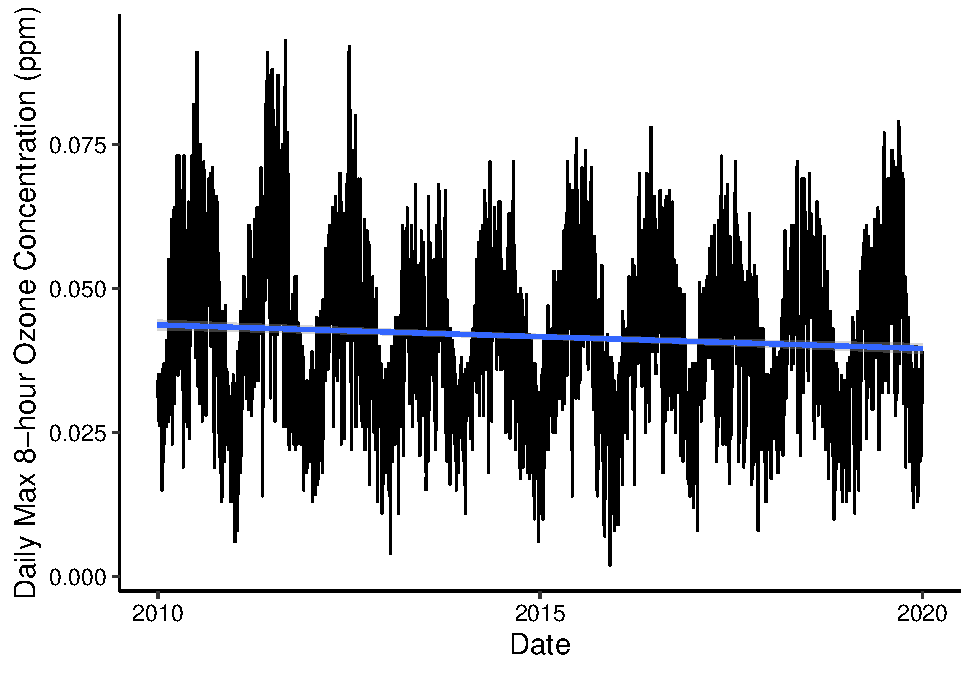
\includegraphics{./-JuilaKirkland-_A08_TimeSeries_files/figure-latex/unnamed-chunk-4-1.pdf}

\begin{quote}
Answer: I see a slight downward trend in ozone concentration over time,
suggesting a gradual decrease in levels from 2010--2019. I also see
clear seasonal variability, with ozone concentrations generally higher
in the summer months and lower in the winter.
\end{quote}

\subsection{Time Series Analysis}\label{time-series-analysis}

Study question: Have ozone concentrations changed over the 2010s at this
station?

\begin{enumerate}
\def\labelenumi{\arabic{enumi}.}
\setcounter{enumi}{7}
\tightlist
\item
  Use a linear interpolation to fill in missing daily data for ozone
  concentration. Why didn't we use a piecewise constant or spline
  interpolation?
\end{enumerate}

\begin{Shaded}
\begin{Highlighting}[]
\CommentTok{\#8}

\NormalTok{GaringerOzone\_clean }\OtherTok{\textless{}{-}} 
\NormalTok{  GaringerOzone }\SpecialCharTok{\%\textgreater{}\%}
  \FunctionTok{mutate}\NormalTok{(}\AttributeTok{Daily.Max.8.hour.Ozone.Concentration.clean =} 
\NormalTok{  zoo}\SpecialCharTok{::}\FunctionTok{na.approx}\NormalTok{(Daily.Max.}\FloatTok{8.}\NormalTok{hour.Ozone.Concentration))}\SpecialCharTok{\%\textgreater{}\%}
  \FunctionTok{select}\NormalTok{ (Date, Daily.Max.}\FloatTok{8.}\NormalTok{hour.Ozone.Concentration.clean)}

\FunctionTok{summary}\NormalTok{(GaringerOzone\_clean}\SpecialCharTok{$}\NormalTok{Daily.Max.}\FloatTok{8.}\NormalTok{hour.Ozone.Concentration.clean)}
\end{Highlighting}
\end{Shaded}

\begin{verbatim}
##    Min. 1st Qu.  Median    Mean 3rd Qu.    Max. 
## 0.00200 0.03200 0.04100 0.04151 0.05100 0.09300
\end{verbatim}

\begin{quote}
Answer: We used linear interpolation because the ozone data show a
generally negative linear trend over time and clear seasonal variation.
Linear interpolation assumes gradual, steady changes between
observations, which fits well for environmental data like ozone that
vary across days and seasons.Using a piecewise constant (``nearest
neighbor'') approach would hold each value constant until the next
observation, creating a step-like pattern that ignores natural seasonal
fluctuations and would make the series look unrealistic.As we learned in
our lesson, spline interpolation would fit smooth curves between points,
but this data does not require that level of smoothing it seems. Linear
interpolatino is a reailstic and best fit way to fill in the missing
values without compromising seaosnal variance or overall trend. It also
works well with datasets with small gaps like this one.
\end{quote}

\begin{enumerate}
\def\labelenumi{\arabic{enumi}.}
\setcounter{enumi}{8}
\tightlist
\item
  Create a new data frame called \texttt{GaringerOzone.monthly} that
  contains aggregated data: mean ozone concentrations for each month. In
  your pipe, you will need to first add columns for year and month to
  form the groupings. In a separate line of code, create a new Date
  column with each month-year combination being set as the first day of
  the month (this is for graphing purposes only)
\end{enumerate}

\begin{Shaded}
\begin{Highlighting}[]
\CommentTok{\#9}

\NormalTok{GaringerOzone\_monthly }\OtherTok{\textless{}{-}}
\NormalTok{  GaringerOzone }\SpecialCharTok{\%\textgreater{}\%} 
   \FunctionTok{mutate}\NormalTok{(}\AttributeTok{Year =} \FunctionTok{year}\NormalTok{(Date),}
        \AttributeTok{Month =} \FunctionTok{month}\NormalTok{(Date)) }\SpecialCharTok{\%\textgreater{}\%}
    \FunctionTok{group\_by}\NormalTok{(Year, Month) }\SpecialCharTok{\%\textgreater{}\%}
    \FunctionTok{summarize}\NormalTok{( }
    \AttributeTok{Month\_Mean\_Ozone =}  \FunctionTok{mean}\NormalTok{(Daily.Max.}\FloatTok{8.}\NormalTok{hour.Ozone.Concentration, }\AttributeTok{na.rm =} \ConstantTok{TRUE}
\NormalTok{    ))}
\end{Highlighting}
\end{Shaded}

\begin{verbatim}
## `summarise()` has grouped output by 'Year'. You can override using the
## `.groups` argument.
\end{verbatim}

\begin{Shaded}
\begin{Highlighting}[]
\NormalTok{GaringerOzone\_monthly\_final }\OtherTok{\textless{}{-}}  
\NormalTok{  GaringerOzone\_monthly }\SpecialCharTok{\%\textgreater{}\%} 
    \FunctionTok{mutate}\NormalTok{(}\AttributeTok{Date =} \FunctionTok{my}\NormalTok{(}\FunctionTok{paste0}\NormalTok{(Month, }\StringTok{"{-}"}\NormalTok{, Year))) }\SpecialCharTok{\%\textgreater{}\%}
    \FunctionTok{select}\NormalTok{(Date, Month\_Mean\_Ozone)}
\end{Highlighting}
\end{Shaded}

\begin{verbatim}
## Adding missing grouping variables: `Year`
\end{verbatim}

\begin{enumerate}
\def\labelenumi{\arabic{enumi}.}
\setcounter{enumi}{9}
\tightlist
\item
  Generate two time series objects. Name the first
  \texttt{GaringerOzone.daily.ts} and base it on the dataframe of daily
  observations. Name the second \texttt{GaringerOzone.monthly.ts} and
  base it on the monthly average ozone values. Be sure that each
  specifies the correct start and end dates and the frequency of the
  time series.
\end{enumerate}

\begin{Shaded}
\begin{Highlighting}[]
\CommentTok{\#10}

\NormalTok{f\_month }\OtherTok{\textless{}{-}} \FunctionTok{month}\NormalTok{(}\FunctionTok{first}\NormalTok{(GaringerOzone\_clean}\SpecialCharTok{$}\NormalTok{Date)) }
\NormalTok{f\_year  }\OtherTok{\textless{}{-}} \FunctionTok{year}\NormalTok{(}\FunctionTok{first}\NormalTok{(GaringerOzone\_clean}\SpecialCharTok{$}\NormalTok{Date))}

\NormalTok{GaringerOzone.daily.ts }\OtherTok{\textless{}{-}} \FunctionTok{ts}\NormalTok{(GaringerOzone\_clean}\SpecialCharTok{$}
\NormalTok{                            Daily.Max.}\FloatTok{8.}\NormalTok{hour.Ozone.Concentration.clean,}
                             \AttributeTok{start =} \FunctionTok{c}\NormalTok{(f\_year, f\_month),}
                             \AttributeTok{frequency =} \DecValTok{365}\NormalTok{)}
                             
\NormalTok{f\_month\_m }\OtherTok{\textless{}{-}} \FunctionTok{month}\NormalTok{(}\FunctionTok{first}\NormalTok{(GaringerOzone\_monthly\_final}\SpecialCharTok{$}\NormalTok{Date))}
\NormalTok{f\_year\_m  }\OtherTok{\textless{}{-}} \FunctionTok{year}\NormalTok{(}\FunctionTok{first}\NormalTok{(GaringerOzone\_monthly\_final}\SpecialCharTok{$}\NormalTok{Date))}

\NormalTok{GaringerOzone.monthly.ts }\OtherTok{\textless{}{-}} \FunctionTok{ts}\NormalTok{(GaringerOzone\_monthly\_final}\SpecialCharTok{$}\NormalTok{Month\_Mean\_Ozone,}
                               \AttributeTok{start =} \FunctionTok{c}\NormalTok{(f\_year\_m, f\_month\_m),}
                               \AttributeTok{frequency =} \DecValTok{12}\NormalTok{)}
\end{Highlighting}
\end{Shaded}

\begin{enumerate}
\def\labelenumi{\arabic{enumi}.}
\setcounter{enumi}{10}
\tightlist
\item
  Decompose the daily and the monthly time series objects and plot the
  components using the \texttt{plot()} function.
\end{enumerate}

\begin{Shaded}
\begin{Highlighting}[]
\CommentTok{\#11}
\NormalTok{GaringerOzone\_daily\_decomp }\OtherTok{\textless{}{-}} \FunctionTok{stl}\NormalTok{(GaringerOzone.daily.ts,}\AttributeTok{s.window =} \StringTok{"periodic"}\NormalTok{)}
\FunctionTok{plot}\NormalTok{(GaringerOzone\_daily\_decomp, }\AttributeTok{main =} \StringTok{"Daily Ozone Decomposition"}\NormalTok{)}
\end{Highlighting}
\end{Shaded}

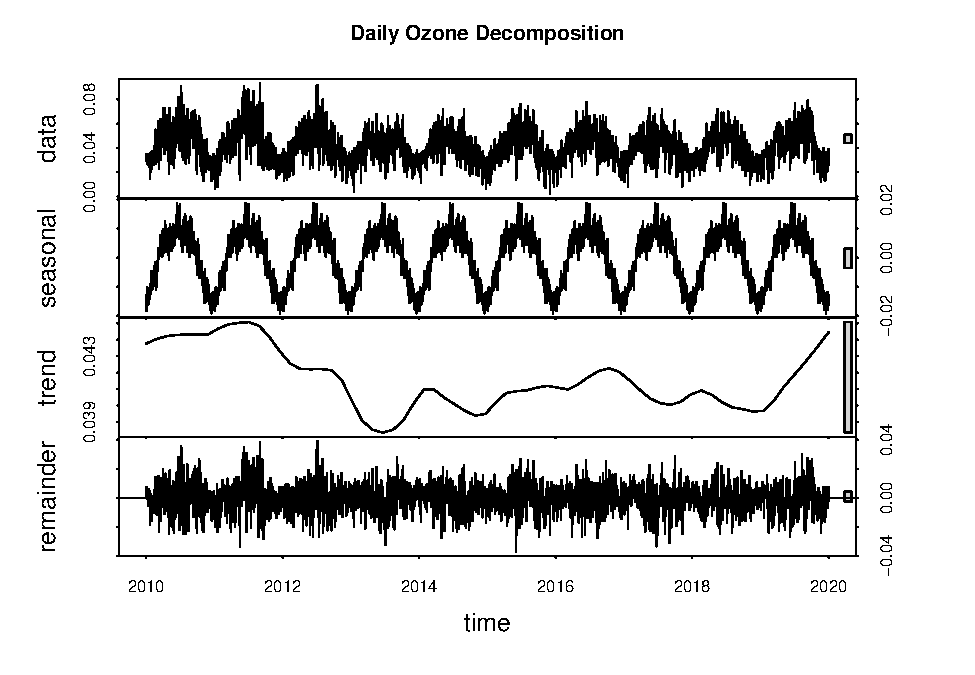
\includegraphics{./-JuilaKirkland-_A08_TimeSeries_files/figure-latex/unnamed-chunk-8-1.pdf}

\begin{Shaded}
\begin{Highlighting}[]
\NormalTok{GaringerOzone\_monthly\_decomp }\OtherTok{\textless{}{-}} \FunctionTok{stl}\NormalTok{(GaringerOzone.monthly.ts,}\AttributeTok{s.window =} \StringTok{"periodic"}\NormalTok{)}
\FunctionTok{plot}\NormalTok{(GaringerOzone\_monthly\_decomp, }\AttributeTok{main =} \StringTok{"Monthly Ozone Decomposition"}\NormalTok{)}
\end{Highlighting}
\end{Shaded}

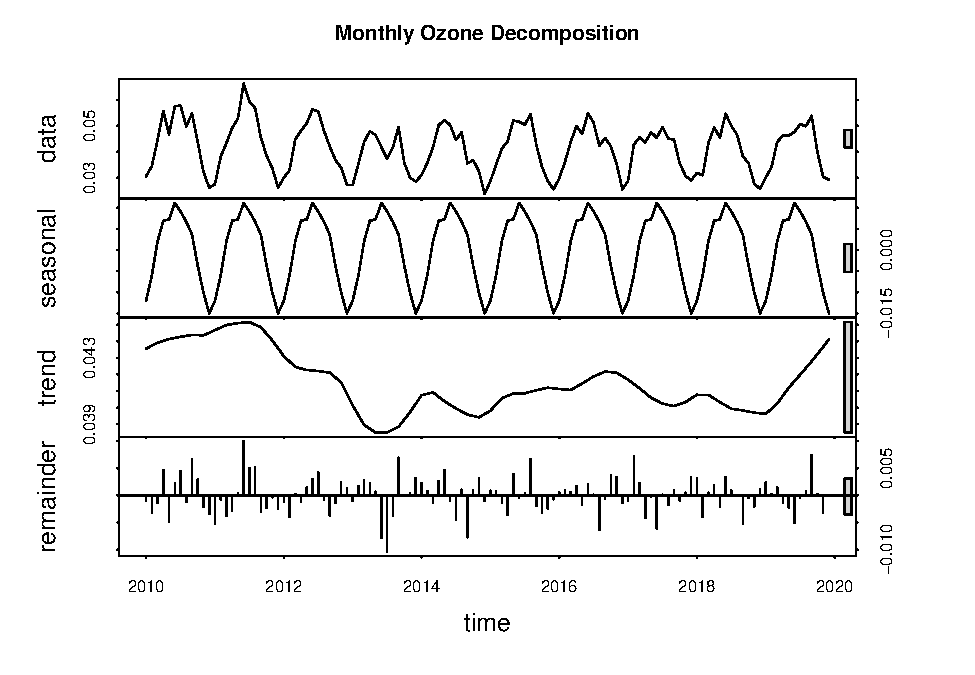
\includegraphics{./-JuilaKirkland-_A08_TimeSeries_files/figure-latex/unnamed-chunk-8-2.pdf}

\begin{enumerate}
\def\labelenumi{\arabic{enumi}.}
\setcounter{enumi}{11}
\tightlist
\item
  Run a monotonic trend analysis for the monthly Ozone series. In this
  case the seasonal Mann-Kendall is most appropriate; why is this?
\end{enumerate}

\begin{Shaded}
\begin{Highlighting}[]
\CommentTok{\#12}

\NormalTok{GaringerOzone\_monthly\_data\_trend }\OtherTok{\textless{}{-}}\NormalTok{ Kendall}\SpecialCharTok{::}\FunctionTok{SeasonalMannKendall}\NormalTok{(GaringerOzone.monthly.ts)}
\FunctionTok{summary}\NormalTok{(GaringerOzone\_monthly\_data\_trend)}
\end{Highlighting}
\end{Shaded}

\begin{verbatim}
## Score =  -88 , Var(Score) = 1498
## denominator =  538.9944
## tau = -0.163, 2-sided pvalue =0.022986
\end{verbatim}

\begin{quote}
Answer: The Seasonal Mann--Kendall test is the most appropriate test for
this dataset because, as shown in the linear regression and
decomposition, the data display clear seasonality. Since the ozone data
is not normally distributed, a non-parametric test is more suitable. The
Seasonal Mann--Kendall test is designed to detect a monotonic trend or,
a consistent upward or downward trend, in data that is seasonal and
unevenly distributed over time.
\end{quote}

\begin{enumerate}
\def\labelenumi{\arabic{enumi}.}
\setcounter{enumi}{12}
\tightlist
\item
  Create a plot depicting mean monthly ozone concentrations over time,
  with both a geom\_point and a geom\_line layer. Edit your axis labels
  accordingly.
\end{enumerate}

\begin{Shaded}
\begin{Highlighting}[]
\CommentTok{\# 13}

\FunctionTok{ggplot}\NormalTok{(GaringerOzone\_monthly\_final, }
\FunctionTok{aes}\NormalTok{(}\AttributeTok{x =}\NormalTok{ Date, }\AttributeTok{y =}\NormalTok{ Month\_Mean\_Ozone)) }\SpecialCharTok{+}
  \FunctionTok{geom\_line}\NormalTok{(}\AttributeTok{color=} \StringTok{"steelblue"}\NormalTok{)}\SpecialCharTok{+}
  \FunctionTok{geom\_point}\NormalTok{(}\AttributeTok{color=} \StringTok{"darkred"}\NormalTok{) }\SpecialCharTok{+}
  \FunctionTok{labs}\NormalTok{(}
  \AttributeTok{x =} \StringTok{"Date"}\NormalTok{, }
  \AttributeTok{y =} \StringTok{"Mean Monthly Ozone Concentration (ppm)"}\NormalTok{,}
  \AttributeTok{title =} \StringTok{"Mean Monthly Ozone Concentration over Time"}
\NormalTok{  )}\SpecialCharTok{+}
\NormalTok{  mytheme }
\end{Highlighting}
\end{Shaded}

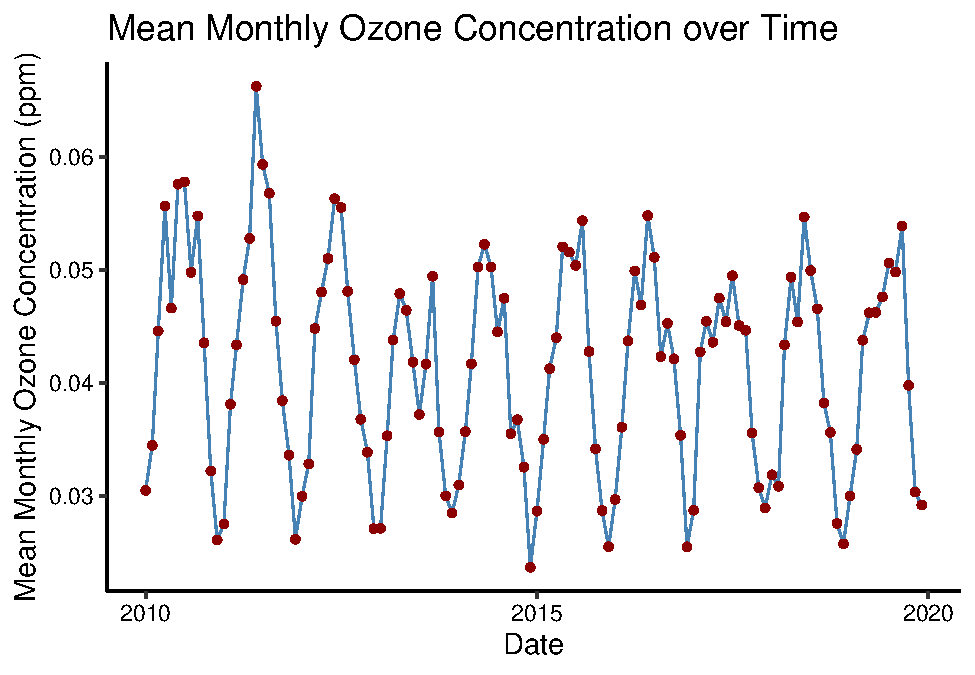
\includegraphics{./-JuilaKirkland-_A08_TimeSeries_files/figure-latex/unnamed-chunk-10-1.pdf}

\begin{enumerate}
\def\labelenumi{\arabic{enumi}.}
\setcounter{enumi}{13}
\tightlist
\item
  To accompany your graph, summarize your results in context of the
  research question. Include output from the statistical test in
  parentheses at the end of your sentence. Feel free to use multiple
  sentences in your interpretation.
\end{enumerate}

\begin{quote}
Answer: An analysis of mean monthly ozone concentrations confirms the
research question: ozone levels at this station did change over the
2010s, showing a statistically significant downward trend. The graph
demonstrates strong seasonal variability over time. The Seasonal
Mann--Kendall test, which accounts for this seasonality, detected an
underlying monotonic decrease in ozone levels (Kendall's tau = −0.163,
p-value = 0.023).
\end{quote}

\begin{enumerate}
\def\labelenumi{\arabic{enumi}.}
\setcounter{enumi}{14}
\item
  Subtract the seasonal component from the
  \texttt{GaringerOzone.monthly.ts}. Hint: Look at how we extracted the
  series components for the EnoDischarge on the lesson Rmd file.
\item
  Run the Mann Kendall test on the non-seasonal Ozone monthly series.
  Compare the results with the ones obtained with the Seasonal Mann
  Kendall on the complete series.
\end{enumerate}

\begin{Shaded}
\begin{Highlighting}[]
\CommentTok{\#15}

\NormalTok{GaringerOzone\_Seasonal\_Component }\OtherTok{\textless{}{-}} 
\NormalTok{GaringerOzone\_monthly\_decomp}\SpecialCharTok{$}\NormalTok{time.series[, }\StringTok{"seasonal"}\NormalTok{]}

\NormalTok{GaringerOzone\_monthly\_noseason\_ts }\OtherTok{\textless{}{-}} 
\NormalTok{GaringerOzone.monthly.ts }\SpecialCharTok{{-}}\NormalTok{ GaringerOzone\_Seasonal\_Component}

\CommentTok{\#16}

\NormalTok{GaringerOzone\_monthly\_data\_trendnoseason }\OtherTok{\textless{}{-}} 
\NormalTok{Kendall}\SpecialCharTok{::}\FunctionTok{MannKendall}\NormalTok{(GaringerOzone\_monthly\_noseason\_ts)}
\FunctionTok{summary}\NormalTok{(GaringerOzone\_monthly\_data\_trendnoseason)}
\end{Highlighting}
\end{Shaded}

\begin{verbatim}
## Score =  -1278 , Var(Score) = 194364.7
## denominator =  7139
## tau = -0.179, 2-sided pvalue =0.0037728
\end{verbatim}

\begin{quote}
Answer: The standard Mann-Kendall test on the non-seasonal time series
yielded a p-value of 0.0038. This is highly significant and even lower
than the p-value from the seasonal test, suggesting the trend is very
unlikely to be due to random chance. Furthermore, the tau value of
-0.179 confirms the downward monotonic trend, reinforcing the conclusion
that ozone levels have significantly decreased over the study period of
the 2010s.
\end{quote}

\end{document}
